% \chapter{\uppercase{Background on Observation-Consistent Inversion} \label{chapter:02}}
% 
% \section{Notation, Terminology, and Assumptions}
% \subsection{Models and Parameters}
% We begin by assuming that a (deterministic) model, denoted by $$\M (u, \param) = 0,$$ is specified to relate observable state variables $u$ to model inputs ({\em parameters}) denoted by the vector $\param\in\RP$.
% The components $\param_\iparam$ may include parameters in either the model operator (e.g. a diffusion coefficient) or input data (e.g. the frequency of a sinusoidal source, initial, or boundary information).
% We let $\pspace$ denote the set of all possible input parameters.
% We assume $\pspace\subset\RP$ is equipped with a (dominating) measure, $\pmeas$ on the Borel $\sa$ $\pborel$, defining the measure space $\Pspace$.
% The solution operator of the model $\M$ then defines a map taking $\param\in\pspace$ to a solution, denoted $u\lam$, to make explicit the dependence on $\param$, which is assumed to be unique.
% 
% However, in real experimental settings we are often unable to fully observe $u\lam$.
% Instead, we often only have access to some finite set of observable scalar quantities.
% For example, in experiments involving the diffusion of heat, we can typically only record the temperature at some small number of pre-specified points in space-time where measurement devices can be positioned.
% 
% \subsection{Quantities of Interest}
% Such observable values of $u\lam$ are mathematically modeled by functionals of the solution, denoted $\qoi_\idata: u\lam \to \RR$.
% The collection of such functionals into a vector defines a {\em Quantity of Interest} (QoI) map.
% Since the solution to the model depends on $\param$, so do the QoI, which motivates the notation
% $$\qlam := \qoi( u\lam ) \in\RD,$$
% to make this dependence on model parameters explicit.
% Furthermore, this convention captures a realistic limitation of an experimental setting, where we may be able to control $\param$ in order to observe $\qlam$, but lack the ability to observe $u\lam$ directly.
% The outputs of the QoI map $\qlam = \data$ are what we refer to as the \emph{data}.
% Similarly, the range of the QoI defines the \emph{data space} $\dspace$, i.e.
% $$\dspace = \qoi(\pspace) \subset \RD$$
% 
% We let $\qspace$ denote the set of possible QoI maps for which it is possible to collect experimental data.
% For example, suppose we can record only a single temperature measurement at any of ten locations in space-time.
% Then $\qspace$ is defined by ten possible QoI maps.
% If we can record any two such measurements, then $\qspace$ is defined by $\binom{10}{2} = 45$ possible maps.
% Observe that $\qspace$ could easily be uncountable\--for example if we were not limited to the spatial locations (or time) at which we could record temperature measurements.
% However, for simplicity, we will only discuss problems where $\qspace$ is finite.
% In the event that we need to compare maps, we adopt the notation $\dspace_{\qoi}$ to emphasize that the data space depends on the choice of QoI map $\qoi$; when the context is clear, we drop the subscript.
% The only assumption on $\qoi$ that we impose throughout this work is that of piecewise-differentiability.
% 
% \subsection{Chapter Outline}
% First, to reflect the order in which these results were researched and developed, we discuss set-based inversion.
% In the interest of clarity of exposition, we have adapted the notation of a sample-based approach developed later to express the construction of the former.
% Consequently, the references cited may require some work translating to match the notation we used.
% Similarities and differences between the two approaches has heretofore avoided formal documentation due to the novelty of the observation-consistent approach, particularly with respect to its use for epistemic uncertainty quantification, and this work serves to lay the groundwork for such a comparison.
% 
% In this chapter, we discuss the issues that arise from the need to numerically approximate the solutions to our inverse problems, and study the implications in \ref{sec:set-error} and \ref{sec:sample-error}.
% Discussion of the impact of sample size are kept to a minimum in this chapter in the interest of restricting the scope of chapter \ref{chapter:03} to the implications for convergence of (consistent) solutions to \eqref{eq:inverse-problem}.
% 
%%%%%%%%%%%%%%%%%%%%%%%%%%%%%%%%%%%%%%%%%%%%%%%%%%%%%%%%%%%%%%%%%%%%%%

%%% THIS GOES TO CH4 NOW %%% 
%\section{Set-Based Inversion for Measures}\label{sec:ch02-set}
% Intro
%To properly summarize the Stochastic Inverse Problem (SIP) and desired solution, we define several measure/probability spaces and refer to the schematic given in Figure \ref{fig:scheme}\---borrowed from \cite{BM17}\---in order to illustrate the steps and spaces required in the formulation and solution of the SIPs we consider herein.
For a more extensive review, we refer the reader to \cite{BBE11}, \cite{BES12}, \cite{BET+14}, and \cite{BM17}.

%%%%%%%%%%%%%%%%%%%%%%%%
\begin{figure}[!h]
\begin{equation}
\underbrace{
\underbrace{
\overbrace{
 \Pspace \xmapsto{\  Q \ } \Dspace
  \xmapsto{\ \dataP \ } (\dspace, \dborel, \dataP)
 }^{
 \text{(S1): Stochastic Inverse Problem (SIP)}
 }
 \xmapsto{\ Q^{-1} \ } (\pspace, \cborel, \contourP)
 }_{
 \text{(S2): Solution to SIP Satisfying Eq. \eqref{eq:dataspace_pushforward_measure}}}
 \xmapsto{\ \set{\PP_\ell}_{\ell\in\mathcal{L}} \ } (\pspace, \pborel, \paramP)
 }
 _{
 \text{(S3): Unique Solution to SIP by Eq.~\eqref{eq:disintegration_measure} and Ansatz}
 }
\end{equation}
\caption{The first step (S1) defines (i)~the formulation of the SIP by specification of the model, (ii)~the measure spaces of parameters and (iii)~observable outputs, and (iv)~the probability measure on the latter. The second step (S2) defines a unique solution to the SIP on the space $\pspace$ equipped with the contour $\sa$ $\cborel$ using the definition of the push-forward measure. In (S3), the Disintegration Theorem and and Ansatz are applied to define a unique solution on the space of interest $(\pspace, \pborel)$ equipped with a probability measure $\paramP$.}
\label{fig:scheme}
\end{figure}


The initial measure/probability spaces involved in the formulation of the SIP are summarized in step (S1) of Fig.~\ref{fig:scheme}, starting with measure space $\Pspace$.

The assumption that $\qoi$ is at least piecewise-differentiable implies the measurability of the QoI map, so that the space $\dspace$ induced by $\qoi$ is equipped with the Borel $\sa$ $\dborel$ [TK - cite textbook].
The ``push-forward'' measure $\dmeas$ on ${(\dspace, \dborel)}$ is defined as
\begin{equation}\label{eq:dataspace_pushforward_measure}
\dmeas (A) = \int_A \, d\dmeas := \int_{\qoi^{-1}(A)} \, d\pmeas = \pmeas \left (\qoi^{-1}(A) \right ) \quad \forall \;  A\in\dborel,
\end{equation}
which defines the measure space $\Dspace$\footnote{When referring to properties of the data space that are not unique to the choice of map used to induce $\dspace$, we will drop the subscript notation and assume the dependence is understood, as expressed in Fig.~\ref{fig:scheme}.}.
The push-forward distribution $\partial \dataP / \partial \mu_D$ is referred to as the \emph{predicted} distribution and is given by the Radon-Nikodym derivative with respect to (the Lebesgue) volume measure $\mu_D$ on ${(\dspace, \dborel)}$

The final step in (S1) involves the specification of a probability measure $\dataP$ on ${(\dspace, \dborel)}$ to model the uncertainty in data.
We colloquially refer to the distribution (given by the Radon-Nikodym derivative $\partial \dataP / \partial \pmeas$) as the \emph{observed} distribution, where $\pmeas$ is taken to be the (Lebesgue) volume measure on ${(\pspace, \pborel)}$.
This leads to the following SIP: determine a probability measure $\paramP$ on ${(\pspace, \pborel)}$ such that the push-forward measure of $\paramP$ matches $\dataP$.

In other words, determine a $\paramP$ satisfying
\begin{equation}\label{eq:inverse_measure}
\paramP \left ( \qoi^{-1}(E)\right ) = \PP_{\dspace}(E) \; \forall \, E \in \dborel.
\end{equation}

We call any such solution $\paramP$ to Eq.~\eqref{eq:inverse_measure} a (measure-theoretic) solution to the SIP.
This equation implies that any solution is uniquely determined on the induced contour $\sa$
\begin{equation}\label{eq:contour_sa}
\cborel = \set{\qoi^{-1}(E) : E \in \dborel } \subset \pborel,
\end{equation}
which is summarized as step (S2) of Fig.~\ref{fig:scheme}.

However, for sets $A \in \pborel \setminus \cborel$, more information is required than is provided in Eq.~\eqref{eq:inverse_measure} in order to determine $\paramP (A)$.
By the Implicit Function Theorem, if $\data \in C^1 (\pspace)$ and we let $\data\in\dspace$ be a fixed datum, $\qoi^{-1}(q)$ exists as a $(\nparams-\ndata)$\--dimensional manifold (possibly piecewise-defined) that we refer to as a \emph{generalized contour} \cite{BET+14}.
These generalized contours can be indexed by a manifold (also possibly piecewise-defined) of dimension $\ndata$ called a \emph{transverse parameterization} that intersects each contour once and only once.
In \cite{BET+14}, it is shown that transverse parameterizations are guaranteed to exist but are in general not unique.

We let $\LL$ denote any particular transverse parameterization.
Each $\ell\in\LL$ corresponds to a unique generalized contour $\CC_\ell \in \pspace$ and each point $\param\in\pspace$ belongs to a unique $\CC_\ell\in\pspace$.
Thus, a transverse parameterization defines a bijection between the manifold $\LL$ and the partitioning of $\pspace$ into generalized contours.
The induced $\sa$ $\cborel$ and this bijection can then be used to define the measurable space $(\LL, \BB_\LL)$.

We denote the projection map $P_\LL : \pspace \to \LL$, and let $\set{\CC_\ell}_{\ell\in\LL}$ represent the family of generalized contours indexed by $\LL$, yielding the associated family of measurable spaces $\set{\left ( \CC_\ell, \BB_{\CC_\ell} \right )}_{\ell\in\LL}{}$.
A Disintegration Theorem [TK - cite] is then leveraged to define a unique decomposition for any $\paramP$ defined on $(\pspace, \pborel)$ as a (marginal) probability measure $\PP_\LL$ on $(\LL, \BB_\LL)$ and a family of (conditional) probability measures $\set{\PP_\ell}_{\ell\in\LL}$ on $\set{\left ( \CC_\ell, \BB_{\CC_\ell} \right )}_{\ell\in\LL}$ such that
\begin{equation}\label{eq:disintegration_measure}
\paramP (A) = \int_{P_\LL(A)} \left ( \int_{P_{\LL}^{-1} (\ell) \cap A}\, d\PP_\ell(\param) \right )\, d\PP_\LL (\ell), \; \forall \; A \in \pborel
\end{equation}

The uniqueness of a probability measure $\paramP$ on ${(\pspace, \cborel)}$ satisfying Eq.~\eqref{eq:inverse_measure} implies the uniqueness of the marginal probability measures $\PP_\LL$ for any particular specification of $\dataP$ on ${(\dspace, \dborel)}$.
The disintegration of Eq.~\eqref{eq:disintegration_measure} implies that a specification of a family of conditional probability measures $\set{P_\ell}_{\ell\in\LL}$ gives us a unique solution to the SIP on ${(\CC_\ell, \BB_{\CC_\ell})}$.

However, the conditional measures cannot be determined by solely by the specification of $\data\in\dspace$.
We follow the work of \cite{BET+14} and adopt the \emph{standard ansatz} determined by the disintegration of the volume measure $\pmeas$ to compute probabilities of sets contained within contour events.
The standard ansatz is given by
\begin{equation}\label{eq:standard_ansatz}
\PP_\ell = \mu_{\CC_\ell} / \mu_{\CC_\ell}(\CC_\ell), \; \forall \; \ell \in \LL,
\end{equation}
where $\mu_{\CC_\ell}$ is the disintegrated volume measure on generalized contour $\CC_\ell$.
Thus, we have defined a unique solution to the SIP on ${(\pspace, \pborel)}$, completing step (S3) in Fig.~\ref{fig:scheme}.

%% \subsubsection{Alternative Derivation Using Bayes' Rule}\label{sec:set_bayes}
In the measure-theoretic approach studied in~\cite{BBE11, BET+14}, Voronoi-cell discretizations of $\pspace$ are used to construct set-valued approximations of the updated measure directly, so we refer to it as the \emph{explicit} approach.
By contrast, sampling from densities is an \emph{implicit} approach, and is discussed in greater detail in \ref{sec:ch02-sample}.
Here, we provide a ``set-based'' derivation of the updated measure to more easily compare to the explicit approximation of the solution given measure in~\cite{BET+14}.

First, we start by observing that if $A, B \subset \pspace$ such that $A = \qoi^{-1}(\qoi(B))$, then we have that $B\subset A$ (the inclusion may be proper).
Therefore, for any probability measure $P$ on $(\pspace, \pborel)$, 
\[
P(B) = P(B|A) \, P(A).
\]
If $P$ is intended to solve the inverse problem, then we are motivated to take
\[
P(A) = \observed (\qoi(A)) = \observed (B),
\]
in the above formula.

We must now determine how to properly define $P(B|A)$. 
We leverage Bayes' Theorem~\cite{Smith} in order to utilize the prior density on contour events.
In other words, we use the prior $\initialP$ on $(\pspace, \pborel)$ and Bayes' Theorem to get
\begin{equation}\label{eq:bayes_full}
P(B|A) = \initialP(B|A) = \frac{ \initialP(A|B) \initialP(B) }{ \initialP(A) },
\end{equation}
and since $B \subset A$, $\initialP(A|B) = 1$, \eqref{eq:bayes_full} simplifies to

\begin{equation}\label{eq:bayes}
\initialP(B|A) = \frac{ \initialP(B) }{ \initialP(A) }.
\end{equation}

Recall from \eqref{eq:predicted} that $\predictedP$ is the push-forward of the prior, giving $\initialP(A) = \predictedP (\qoi(A)) = \predictedP \left (\qoi(B)\right )$, which then gives the following set-valued ``solution'' to the stochastic inverse problem:
\begin{equation}\label{eq:sip_sol_cont}
\updatedP(B) := \begin{cases}
\initialP(B) \frac{ \observed(B) }{ \predictedP \left (\qoi(B)\right ) ) } & \text{ if } \initialP(B) > 0,\\
0 & \text{ otherwise}.
\end{cases}
\end{equation}

This set-valued update is only a solution on certain (sub-)$\sigma$-algebras of $\pborel$. 
Nonetheless, we can form explicit approximations to the update, e.g. as done in~\cite{BET+14, BES12, BBE11}. 
In other words, an Ansatz is used in place of the prior; it serves the same purpose to distribute probabilities in directions not informed by the QoI map.

However, such an explicit approach requires an approximation of \emph{events in $\pborel$}. 
This is in direct contrast to the numerical approximation of the density $\updated$ that only requires approximation of $\predicted$.
Since we often expect the dimension of $\dspace$ to be less than the dimension of $\pspace$, this can prove to be a significant numerical advantage for the ``implicit'' approximation given by the updated probability density function. 

% Numerical Approximation
%\subsection{Numerical Approximation and Analysis}\label{sec:set-algorithm}
We present a non-intrusive algorithm based on Monte-Carlo sampling\---initially introduced in \cite{BET+14} and further analyzed in \cite{BET+14-arxiv}\---that is structured in four stages (written as four independent for-loops) that are linked to the stages in Fig.~\ref{fig:scheme}.
We direct the interested reader to \cite{BET+14-arxiv} for more detailed information and analysis of this algorithm, e.g., on the requirement of a sampler being ``$\pborel$-consistent'' to ensure convergence.


\begin{algorithm}[hbtp]
\DontPrintSemicolon
Choose a discretization partition $\set{D_\idisc}_{\idisc=1}^{\ndiscs}$ of $\dspace$.\\
	\For{$\idisc = 1, \hdots, \ndiscs$}{
			Compute $p_{\dspace, \idisc} = \dataP(D_\idisc)$.
	}
	Choose samples $\set{\param^{(\iparam)}}_{\iparam=1}^{\nsamps} \subset \pspace$, which implicitly defines a Voronoi-cell partition $\set{\VV_\iparam}_{\iparam=1}^{\nsamps}$ of $\pspace$.\\
	\For{$\iparam = 1, \hdots, \nsamps$}{
	Compute $\qoi_\iparam = \qoi(\param^{(\iparam)})$.\\
	Let $\OO_\idisc = \set{\iparam: \qoi_\iparam \in D_\idisc}$.\\
	Compute approximations $V_\iparam \approx \pmeas (\VV_\iparam)$.
	}
	\For{$\idisc = 1, \hdots, \ndiscs$}{
	Compute $\CC_\idisc = \set{\iparam:Q_\iparam \in D_\idisc}$.
	}
	\For{$\iparam = 1, \hdots, \nsamps$}{
	Compute $p_{\pspace, \iparam} = \left ( V_\iparam / \sum_{j\in \CC_{\OO_\iparam} } V_j \right ) p_{\dspace, \OO_\iparam}$.
	}
	For any $A\in \pborel$, compute
	\begin{equation}
	\PP_{\pspace, \ndiscs, \nsamps} (A) = \sum_{\iparam=1}^\nsamps p_{\pspace, \iparam} \Chi_{\VV_\iparam} (A)
	\end{equation}
 \caption{Numerical Approximation of the Inverse Density}
 \label{alg:inv_density}
\end{algorithm}


The first two stages correspond to formulating the discretized version of the SIP given in step (S1) in Fig.~\ref{fig:scheme}.
We first discretize the probability space $\Ospace$.
Then, we simultaneously discretize the measure space $(\pspace, \pborel, \pmeas)$ and construct a simple-function approximation to the map $\qoi$.
These stages introduce the primary sources of error, and the third and fourth stages may be thought of as solving the discretized SIP exactly.
The samples that are used to describe $\pspace$ implicitly define a set of Voronoi cells $\set{\VV_\iparam}_{\iparam=1}^{\nsamps}$, which can be seen in Figure~\ref{fig:voronoi_cells}.
Each sample set defines a fundamentally different geometry.

\begin{figure}[ht]
\centering
	\begin{minipage}{.475\textwidth}
		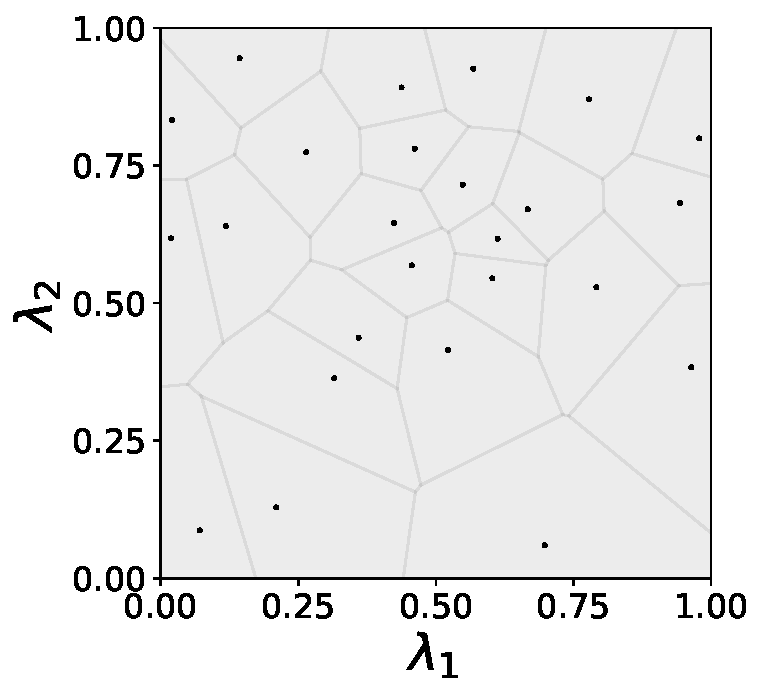
\includegraphics[width=\linewidth]{./images/voronoi_diagrams/voronoi_diagram_N25_r0}
	\end{minipage}
\caption{
Voronoi-cell discretization (partition) induced by $\nsamps = 25 $ uniform i.i.d.~random samples in $\pspace = [0,1]^2$.
}
\label{fig:voronoi_cells}
\end{figure}

The third stage then identifies the collection of Voronoi cells in $\pspace$ that approximate the contour events in $\cborel$ defined by $\qoi^{-1}(D_\idisc)$ for $\idisc=1,\hdots,\ndiscs$. This allows us to formulate the consistent solution to the discretized SIP on $(\pspace, \cborel, \contourP)$ as illustrated in step (S2) of Fig.~\ref{fig:scheme}.
Finally, the fourth stage\---associated with step (S3) in Fig.~\ref{fig:scheme}\---uses a discrete version of the ansatz to approximate the probability of $\VV_\iparam$ for $\iparam=1,\dots,\nsamps$.
This results in an approximate probability measure, denoted by $\PP_{\pspace, \ndiscs, \nsamps}$, which produces the same probability estimates for events $A$ and $A\setminus \set{ \param^{(\iparam)} }_{\iparam=1}^\nsamps$, which are identical almost everywhere with respect to $\pmeas$.

Note that Algorithm~\ref{alg:inv_density} makes no mention of the method by which the samples $\set{ \param^{(\iparam)} }_{\iparam=1}^{\nsamps}$ were generated or sets in $\set{D_\idisc}_{\idisc=1}^{\ndiscs}$ are chosen.
$\set{ \param^{(\iparam)} }_{\iparam=1}^{\nsamps}$ may be generated using uniform random sampling, latin hypercube sampling, or even regular grids.
A thorough discussion of the choices involved in making such decisions is beyond the scope of this work, though we touch briefly on the discretization of $\dspace$ below.


% Descriptions of Error
%\subsection{Descriptions of Error}\label{sec:set-error}

Recall that we assumed $\dataP$ is absolutely continuous with respect to $\dmeas$, which allows us to describe $\dataP$ with a density $\rho_\dspace$. Then, for any partition $\set{D_\idisc}_{\idisc=1}^{\ndiscs}$ of $\dspace$,
\[
\dataP (D_\idisc) = \int_{D_\idisc} \rho_\dspace \, \dmeas, \quad \text{ for } \idisc = 1, \hdots, \ndiscs.
\]

We often use Monte Carlo approximations to compute the approximations $p_{\dspace, \idisc}=\dataP(D_\idisc)$ in the first for-loop in Algorithm~\ref{alg:inv_density}.
These samples are generated on $\dspace$ and do not require numerical solutions to the model.
We therefore assume that for any discretization of $\dspace$, these approximations can be made sufficiently accurate and neglect the error in this computation.

We denote the exact solution to the SIP associated with this partitioning of $\dspace$ by $\PP_{\pspace, \ndiscs}$.
In situations where $\qoi(\param^{(\iparam)})$ is estimated (e.g. by application of a functional on a finite-element solution to a PDE), the approximate solutions to the SIP given in the final for-loop of Algorithm~\ref{alg:inv_density} are denoted by $\PP_{\pspace, \ndiscs, \nsamps, h}$.
Here, the $h$ is in reference to a mesh or other numerical parameter that determines the accuracy of the numerical solution $u_h(\param^{(\iparam)})\approx u(\param^{(\iparam)})$, and subsequently the accuracy in the computations of $\qoi_\iparam = \qoi(\param^{(\iparam)})$ in Algorithm~\ref{alg:inv_density}.

We assume that $h$ is tunable so that for any $A\in \pborel$,
\[
\lim\limits_{h \downarrow 0} \PP_{\pspace, \ndiscs, \nsamps, \imesh} (A) = \PP_{\pspace, \ndiscs, \nsamps} (A).
\]
It is possible to prove the convergence of $\PP_{\pspace, \ndiscs, \nsamps, \imesh} (A) \to \paramP (A)$ for some $A\in \pborel$ and on estimating the error in $\PP_{\pspace, \ndiscs, \nsamps, h}(A)$.
For example, in \cite{BGE+15}, adjoint-based a posteriori estimates in the computed QoI are combined with a statistical analysis to both estimate and bound the error in $\PP_{\pspace, \ndiscs, \nsamps, \imesh} (A)$.
In [TK - cite ISNME 2019], adjoints are used to compute both error and derivative estimates of $\qoi(\param^{(\iparam)})$ to improve the accuracy in $\PP_{\pspace, \ndiscs, \nsamps, \imesh} (A)$.
However, no work has to date fully explored the \emph{convergence rates} of Algorithm \ref{alg:inv_density}.
Furthermore, no work has yet to establish that these rates are independent of the choice of QoI map despite other studies establishing that the absolute error is very much affected by the geometric properties of the QoI maps [TK - cite Lindley + Butler].

In order to study convergence, we need to define a notion of distance on the space of probability measures on $\pspace$, which we denote by $\PPspace$.
% There are many choices available to us and we discuss several useful metrics on $\paramP$ in Section~\ref{sec:metrics}.
We use the Total Variation metric (TV) throughout this work, but for the time being, let $d$ represent any metric on $\PPspace$.

Then, by repeated application of the triangle inequality,
\begin{equation}
\label{eq:set-triangleineq}
d(\PP_{\pspace, \ndiscs, \nsamps, h}, \paramP) \leq
\underset{ \text{(E1)} }{\underbrace{d(\PP_{\pspace, \ndiscs, \nsamps, h},\PP_{\pspace, \ndiscs, \nsamps})}} +
\underset{ \text{(E2)} }{\underbrace{d(\PP_{\pspace, \ndiscs, \nsamps}, \PP_{\pspace, \ndiscs}) }}+
\underset{ \text{(E3)} }{\underbrace{d(\PP_{\pspace, \ndiscs}, \paramP) }}.
\end{equation}

The term (E1) describes the effect of the error in the numerically evaluated $\qoi_\iparam$ on the solution to the SIP.
The term (E2) describes the effect of finite sampling error in $\pspace$ on the solution to the SIP and (E3) describes the effect of discretization error of $\dataP$ on the solution to the SIP.


%%%% END OF WHAT IS KEPT %%%


% Example
%\subsection{Example}\label{sec:set-example}

TK - Introduce, 2D identity map, known observed (square in center with area 1/100, i.e. density value of 100).

\begin{python}
"""
Set up and solve problem with identity map
"""
# import libraries
import bet.sample as sample
import bet.sampling.basicSampling as bsam
import bet.calculateP.simpleFunP as simpleFunP
import bet.calculateP.calculateP as calculateP
import numpy as np
import scipy.stats as sstats

# define input space parameters and model to instantiate sampler object
dimension = 2
numSamples = 100
I = np.eye(dimension)
def model(input_samples):
        return (I@input_samples.T).T
sampler = bsam.sampler(model)

# instantiate objects that hold input/output samples
# default random sample set is uniform over unit domain (normalized space)
input_set = input_samples = bsam.random_sample_set('r',input_obj=dimension, num_samples=numSamples)
param_ref = np.array([0.5, 0.5])
input_set.set_reference_value(param_ref)

# Estimate volumes of Voronoi cells associated with the parameter samples
if MC_assumption is False:
    input_samples.estimate_volume(n_mc_points=5E4)
else:
    input_samples.estimate_volume_mc()

# input_set = bsam.regular_sample_set(input_obj=dimension, num_samples_per_dim=49)
disc = sampler.compute_QoI_and_create_discretization(input_sample_set=input_set)
Qref = disc.get_output().get_reference_value()
print('Reference Value:', param_ref, 'maps to', Qref)

# define inverse problem
disc_1 = disc.copy()
simpleFunP.regular_partition_uniform_distribution_rectangle_size(
        data_set=disc_1, Q_ref=Qref, rect_size=0.2,
        cells_per_dimension = 1)
calculateP.prob(disc_1)

# compare with higher-fidelity discretization of output space
disc_2 = disc.copy()
simpleFunP.regular_partition_uniform_distribution_rectangle_size(
        data_set=disc_2, Q_ref=Qref, rect_size=0.2,
        cells_per_dimension = 2)
calculateP.prob(disc_2)

\end{python}

Note that there is no need to explictly call {\tt disc.compute\_pushforward()}, (or \pythoninline{disc.compute_predicted()}) since it is computed automatically if none have been previously constructed.
When \pythoninline{disc.updated_pdf()} is called, densities are evaluated at the initial set of $\nsamps$ random samples, and stored in \pythoninline{disc._input_sample_set._densities}.
However, the function \pythoninline{disc.predicted_pdf()} is capable of evaluating the solution at any new set of samples (provided a model is available/equipped to the discretization), something we leverage for plotting on a regular grid.

Once our four discretization objects \pythoninline{disc}, \pythoninline{disc_a}, \pythoninline{disc_b} and \pythoninline{disc_c} have been generated, we can use some utility plotting functions to compare the densities:

\begin{python}
"""
Plotting code to generate figures.
"""
# define plotting parameters
nbins = 50
xmn, xmx = 0.25, 0.75
ymn, ymx = 0.25, 0.75
xi, yi = np.mgrid[xmn:xmx:nbins*1j, ymn:ymx:nbins*1j]

# plotting functions computes nearest-neighbors to
# the regular grid of samples.
plot_2d_comparison(xi, yi, disc_1, disc_2,
                   '$M=1, N=%d$'%(numSamples),
                   '$M=4, N=%d$'%(numSamples))
\end{python}

\begin{figure}[ht]
\begin{minipage}{.975\textwidth}
  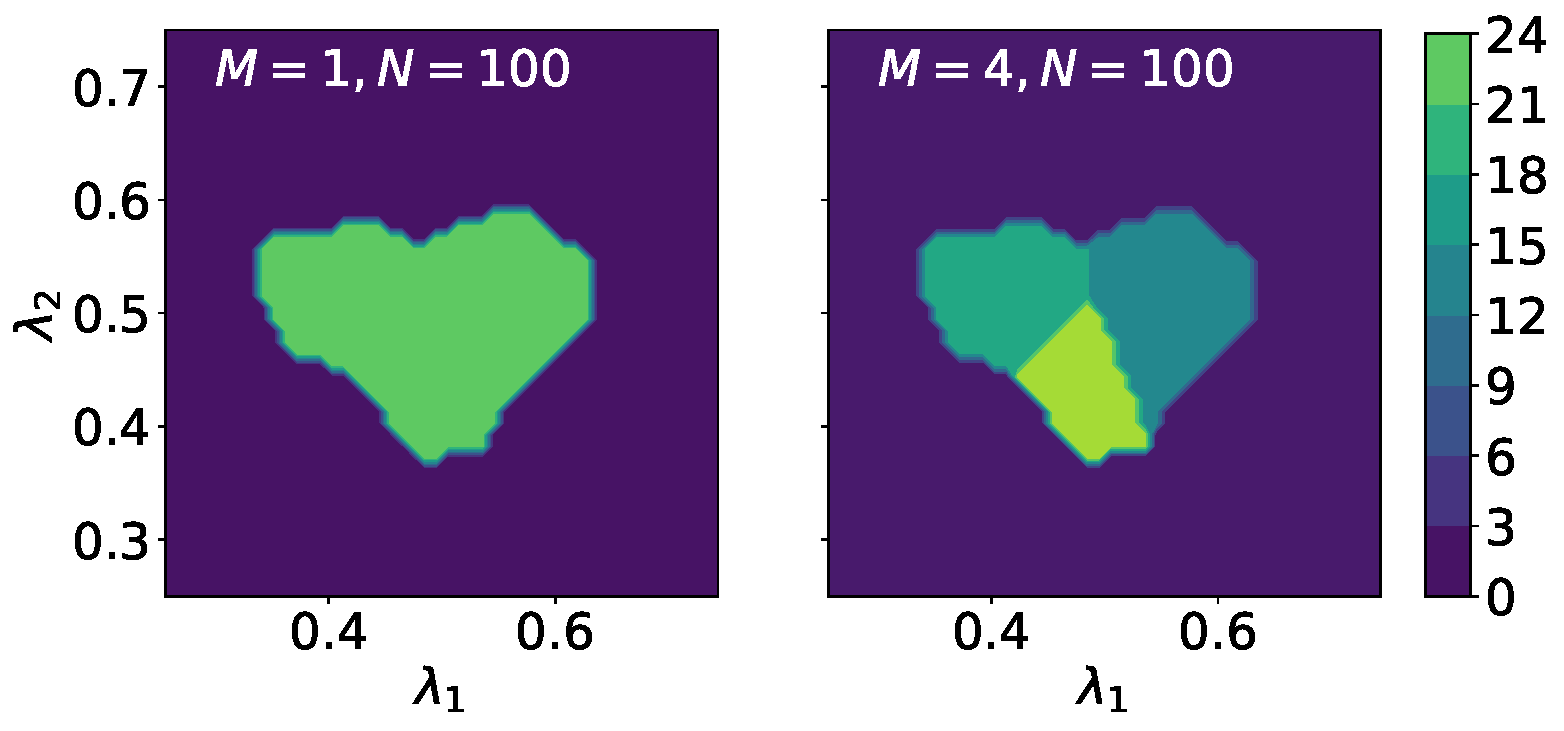
\includegraphics[width=\linewidth]{./examples/identity/set/M1-N100_N100-vs-M4-N100_N100.pdf}
\end{minipage}
\caption{
$\nsamps=100$ were used to discretize $\pspace$ and $\ndiscs=1, 4$ (left/right) were used to discretize $\dspace$.
The latter was chosen to visualize the geometry of describing $\pspace$ with $\pborel$.
}
\label{fig:ex:identity_set_1E2}
\end{figure}

We have chosen a uniform density to describe the uncertainty in our output space.
Any value that is within $0.1$ to the left and right of the reference value \pythoninline{Qref = [0.5, 0.5]} in each dimension is treated as equally likely.
This was done so that using $\ndiscs = 1$ samples to discretize $\dspace$ would fully characterize the characteristic function density representing this uncertainty.
The inverse image of this set is a characteristic function defined on $\pborel$, so errors will exist in particular at the boundaries of the region.

The fundamental challenge with the set-based approach is linked to the geometry of the induced Voronoi-cell tesselation on $\pspace$.
With only $\nsamps = 100$ samples, we see in \ref{fig:ex:identity_set_1E2} that the region (which is supposed to be a square) hardly represents one.
There is ample variation in the shape parameters of the induced sets $\VV_\iparam$ when so few samples are used.
It is possible to ``get lucky'' with the aligning of boundaries between the true target density $\Chi_{[0.4, 0.6]^2}$, but the Figure is representative of the difficulty of using $\nsamps = 100$ random samples to describe a geometry.
With $\nsamps = 1000$, there are usually still significant differences in the symmetric difference of approximated and true supports of the densities.

Below, we demonstrate the use of more samples to resolve the geometry of the desired set.
\begin{figure}[ht]
\begin{minipage}{.975\textwidth}
  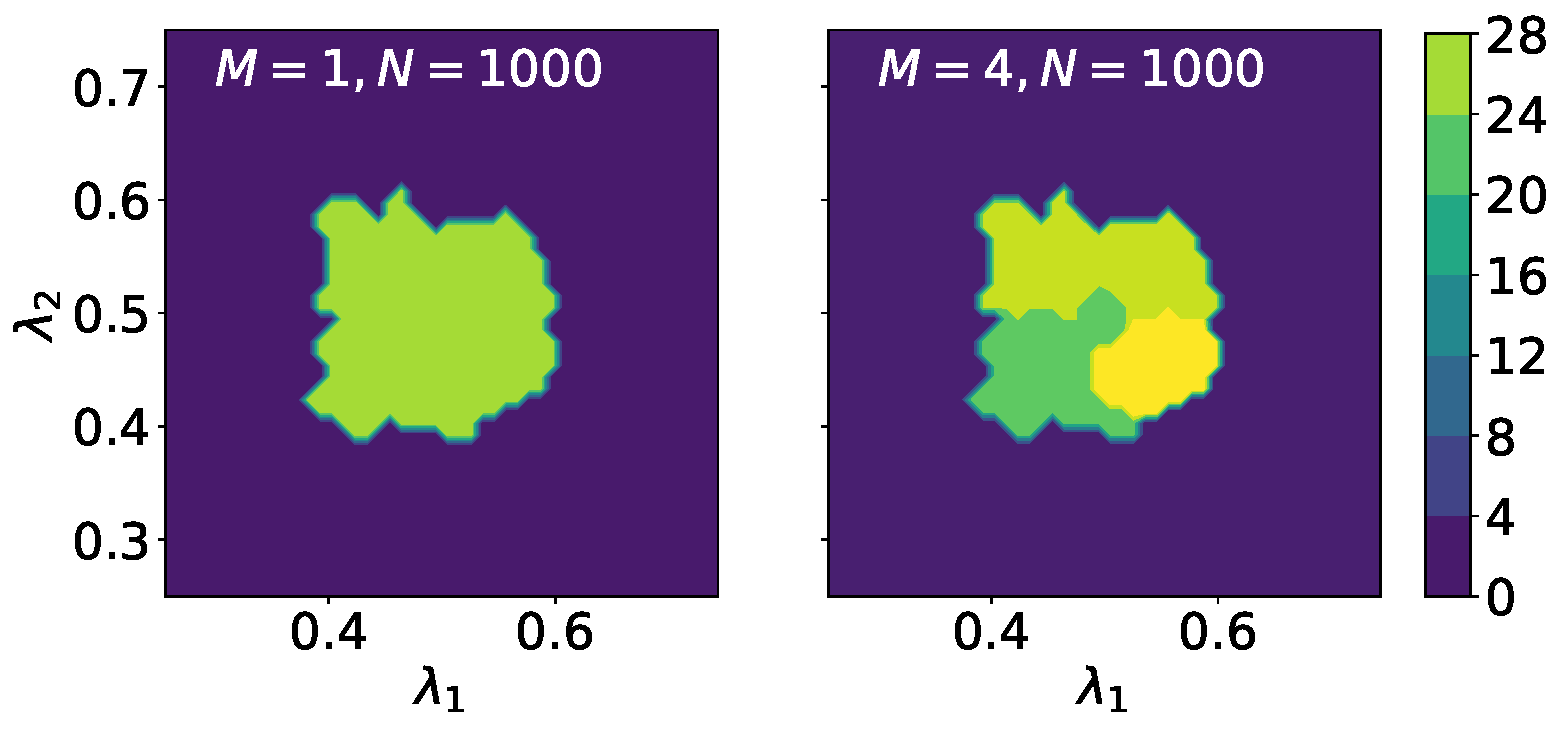
\includegraphics[width=\linewidth]{./examples/identity/set/M1-N1000_N1000-vs-M4-N1000_N1000.pdf}
  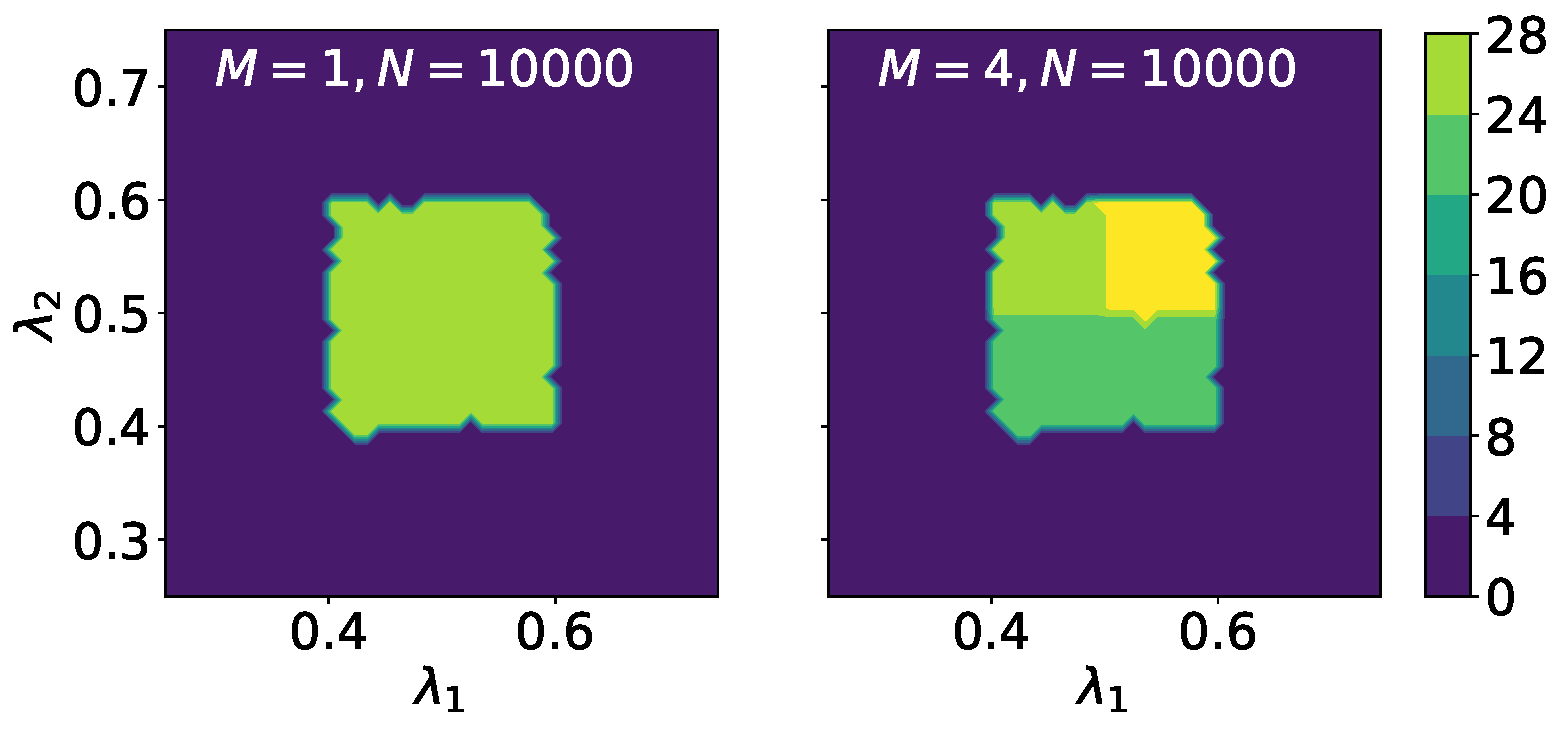
\includegraphics[width=\linewidth]{./examples/identity/set/M1-N10000_N10000-vs-M4-N10000_N10000.pdf}
\end{minipage}
\caption{
(Top):$\nsamps=1,000$ were used to discretize $\pspace$ and $\ndiscs=1, 4$ (left/right) were used to discretize $\dspace$.
(Bottom): The same, except with $\nsamps=10,000$, where we finally begin to see something resembling the correct correct geometry.
}
\label{fig:ex:identity_set_1E3_1E4}
\end{figure}
\FloatBarrier

We remark on the fact that in this particular situation, $\ndiscs = 1$ is a ``correct'' choice for the probability measure chosen, and $\ndiscs = 4$ actually introduces errors.
The reason that the latter solutions have different values inside of the support of $\PPspace$

%\FloatBarrier

%%%%%%%%%%%%%%%%%%%%%%%%%%%%%%%%%%%%%%%%%%%%%%%%%%%%%%%%%%%%%%%%%%%%%%
% \pagebreak
%\section{Sample-Based Inversion for Measures}\label{sec:ch02-sample}

%% Intro
% In [TK - reference] it was shown that an equivalent derivation to the same set-based solution to the SIP presented in \ref{sec:ch02-set} could be achieved with the following form:

\begin{equation}
\dciP
\end{equation}


This equation presents on the left-hand side the solution to the SIP, referred to as the updated measure $\updatedP$, which is equal to a scaling of an initial probabaility measure $\initialP$ by a ratio of observed $\observedP$ to predicted $\predictedP$ measures.
Taking the Radon-Nikodym derivatives of each of the respective terms, we can arrive at a more natural distribution-based description of the solution:

\begin{equation}
\begin{split}
\dci\\
\dciD
\end{split}
\end{equation}

The initial density $\initial$ encodes the information that the ansatz played in \ref{sec:ch02-set}, which is to assign relative probabilities among points which belong to the same equivalence class of solutions.

% \FloatBarrier
%% Numerical Approximation
% \subsection{Numerical Approximation and Analysis}\label{sec:sample-algorithm}

[TK - Algorithm goes here]

picture of pushforward given different number of samples, overview of KDE

% \FloatBarrier
%% Descriptions of Error
% \subsection{Descriptions of Error}\label{sec:sample-error}

[TK - this section below is still a bit rough, but the ideas are starting to get laid out]

The source of approximation error in the sample-based approach comes from a fundamentally different source.
We transfer the burden of responsibility for accurate approximation towards the data space instead of the parameter space.
To estimate a push forward distribution, samples that are drawn from the initial density represent our total model evaluation budget.
For the sample-based approach, it is important to ask: \emph{Is the number of samples still important for accurate approximation?}
We demonstrate that the answer is yes, but the dependence is shifted from the parameter space to the data space, which is often of a lower dimension, which requires less samples to accurately approximate due to the dependence of density approximation on dimension.
We construct a similar triangle inequality as in \ref{sec:set-error}, but the sources of error now bear different interpretations.

We have by repeated application of the triangle inequality that

\begin{equation}
\label{eq:sample-triangleineq}
d(\PP_{\pspace, \ndiscs, \nsamps, h}, \paramP) \leq
\underset{ \text{(E1)} }{\underbrace{d(\PP_{\pspace, \ndiscs, \nsamps, h},\PP_{\pspace, \ndiscs, \nsamps})}} +
\underset{ \text{(E2)} }{\underbrace{d(\PP_{\pspace, \ndiscs, \nsamps}, \PP_{\pspace, \ndiscs}) }}+
\underset{ \text{(E3)} }{\underbrace{d(\PP_{\pspace, \ndiscs}, \paramP) }}.
\end{equation}


Since there is no error in approximating the specification of an observed distribution, the only sources of error are those that arise from inaccurately assigning probability to samples in the denominator of equation \eqref{eq:updated-density} (i.e., approximating the predicted distribution/measure).
The merits of different density approximation methods is beyond the scope of this work, but we provide a brief review of the challenges involved with approximating distributions in high dimensions.
In some sense there is a need to balance the size of the data space and the number of samples available to characterize it.
If model evaluation is cheap, larger data spaces can be constructed to be more informative and have better geometric properties for approximating a solution.
If model evaluations are limited, or perhaps already exhausted, then there may be motivation to pose a one-dimensional problem because it minimizes error in the predicted distribution due to dimension.
We are motivated to minimize the difference in dimension between input output space but as the dimension of the day is best grows, our approximation error at a fixed sample size grow out of proportion.

We summarize some illustrative results for clarification from \cite{Silverman} on the topic of one-dimensional Gaussian density estimation.
The table in \ref{table:silverman} shows the required sample size as a function of dimension required to ensure that the relative mean square error at zero is less than 0.1 (which says nothing of global accuracy).

\begin{figure}
  \begin{tabular}{ l | l }
  \hline \\ Dimensionality & Required Sample Size\\ \hline
  1  & 4\\
  2  & 19\\
  3  & 67\\
  4  & 223\\
  5  & 768\\
  6  & 2 790\\
  7  & 10 700\\
  8  & 43 700\\
  9  & 187 000\\
  10 & 842 000\\ \hline
  \end{tabular}
\caption{Sample size required (accurate to about 3 significant figures) to ensure that the relative mean square error at zero is less than $0.1$, when estimating a standard multivariate normal density using a normal kernel and the window width that minimizes the mean square error at zero.}
\label{table:silverman}
\end{figure}

To achieve this tolerance of 0.1 for a integrated square error $E \int (\hat{f} - f)^2 / \inf f^2$ would require approximately $1.7$ times the samples shown in \ref{table:silverman} for dimensions up to 10 \cite{Silverman}.
The sample sizes required grow even larger for global measures of accuracy, which are fortunately rarely required to achieve in practice due to the nature of $\observed$ assigning probability over only a region of $\predicted$.

% \FloatBarrier
%% Example
% \subsection{Example}\label{sec:sample-example}

We have observed how the set-based approach to solving inverse problems can lead to errors in approximating measures, particularly around the boundaries of the solution set.
The sample-based approach that we summarized above does not rely on Voronoi-cell approximations of contour events, instead assigning probability to random samples drawn from an initial density.

We demonstrate that for estimating a uniform density over a subset of the initial parameter space, the sample-based approach is able to more accurately approximate it at a given sample size.
The reason for this is that the approach has a different source of error, involving estimating to push forward of the initial density.

We are interested in studying how our ability to estimate a uniform density is impacted by the number of samples drawn from the initial density.
We form an inverse problem with the identity map an standard uniform initial densities, with observed densities being uniform over $[0.4, 0.6]^2$, representing a hundred-fold reduction in uncertainty when the problem is solved

We solve the same problem as before but use a uniform initial density in place of a uniform ansatz.
We sample $N=100$, $1,000$ and $10,000$ samples from the initial density and use Gaussian kernel density estimation to approximate the denominator in Eq [TK - eq], and show the resulting updated densities in Figure~\ref{fig:ex:identity_sampling_approx}.

Observe that the support of the updated density matches the solution of the previous inverse problem but is much more accurately approximated.
Gone are the jagged edges that we saw before, replaced by clean squares.
The relative probability is assigned within the support are also more similar to one another, something we demonstrate in Figure~\ref{fig:identity_sampling_conditionals}, which shows conditional densities along the unit directions through the center of the domain.

\begin{figure}[ht]
\begin{minipage}{.975\textwidth}
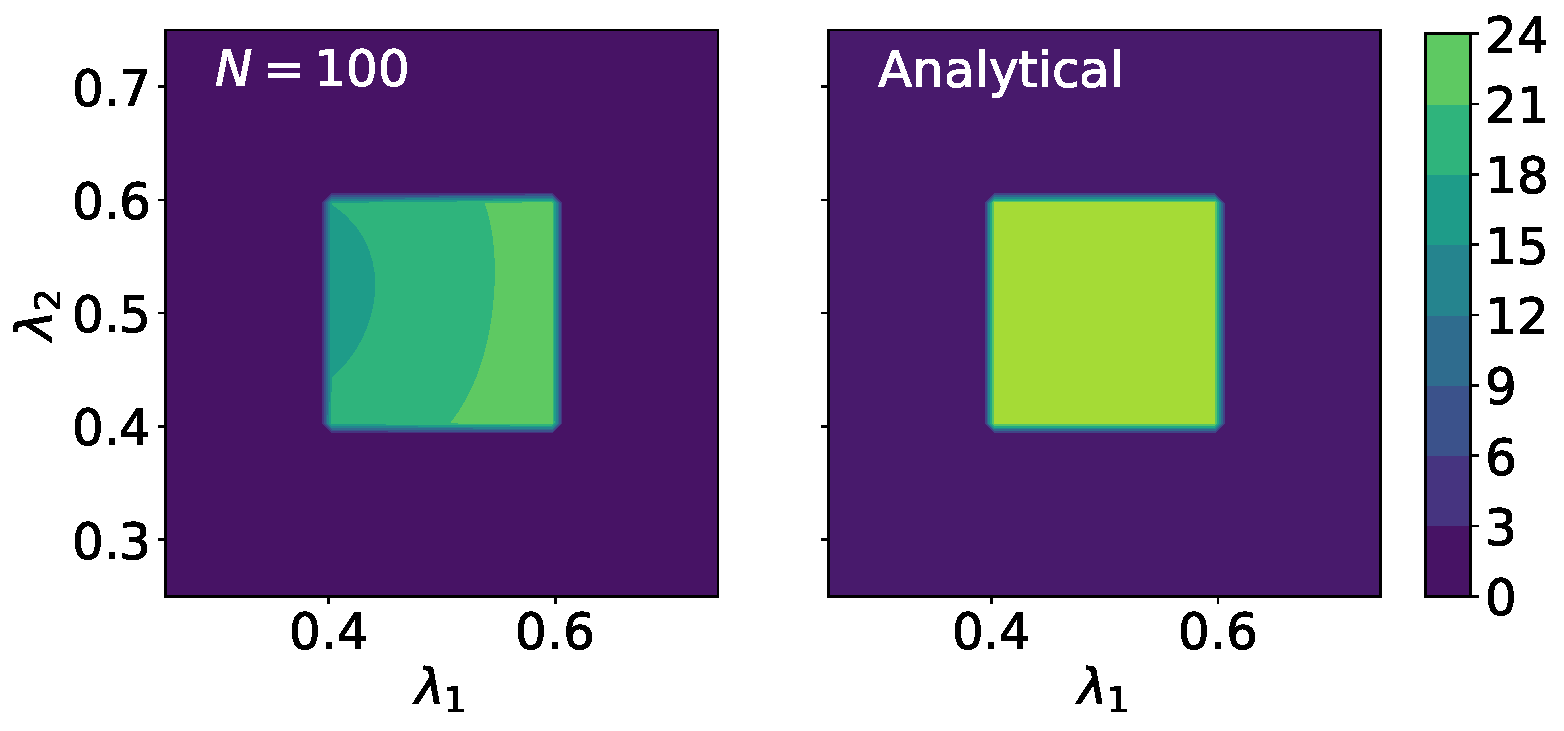
\includegraphics[width=\linewidth]{./examples/identity/samp/N100_N100-vs-Analytical_N100.pdf}
\end{minipage}
\caption{
(Left): $\nsamps=100$ were used to construct the predicted distribution $\predicted$.
(Right): By specifying an analytical $\predicted$, the effect of using $\nsamps$ to approximate a pushforward distribution disappears. The problem can be fully specified in BET without any random sampling.
}
\label{fig:ex:identity_sampling_exact}
\end{figure}

\begin{figure}[ht]
\begin{minipage}{.975\textwidth}
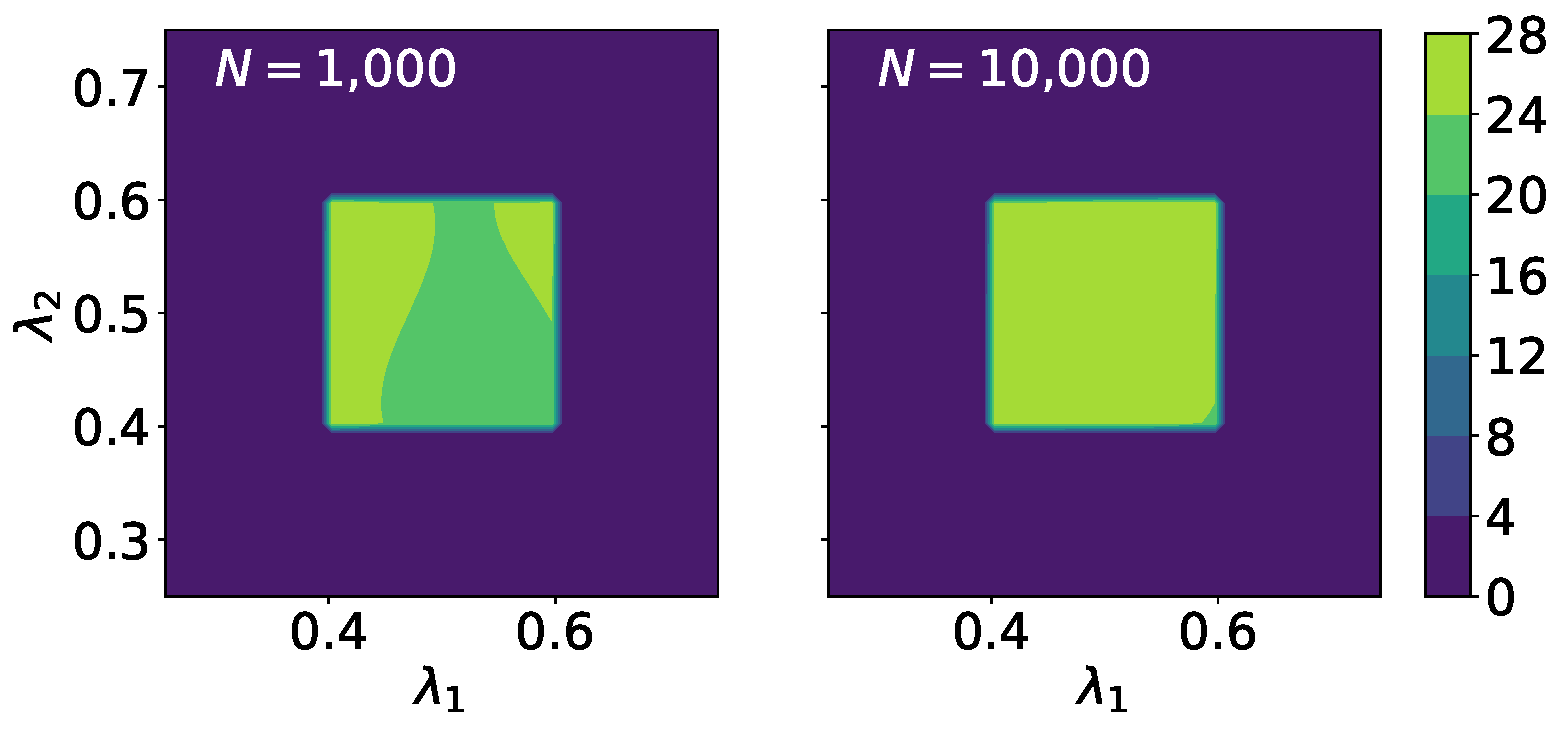
\includegraphics[width=\linewidth]{./examples/identity/samp/N1-000_N1000-vs-N10-000_N10000.pdf}
\end{minipage}
\caption{
$\nsamps=1,000$ (left) and $\nsamps=10,000$(right) were used to construct the predicted distribution $\predicted$.
There is no signficant error in estimating the support of the distribution, only the density approximation itself.
}
\label{fig:ex:identity_sampling_approx}
\end{figure}

\begin{figure}[ht]
\centering
% N = 1E2
\begin{minipage}{.975\textwidth}
		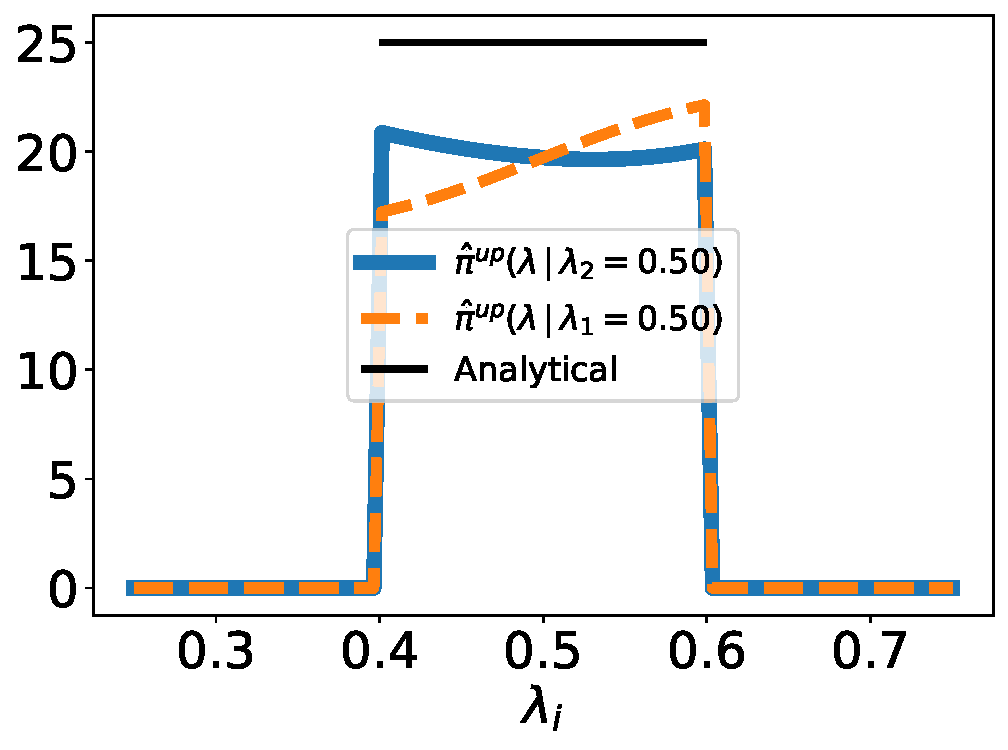
\includegraphics[width=0.5\linewidth]{./examples/identity/samp/identity_1d_conditionals_50E-2_N100_approx.pdf}
    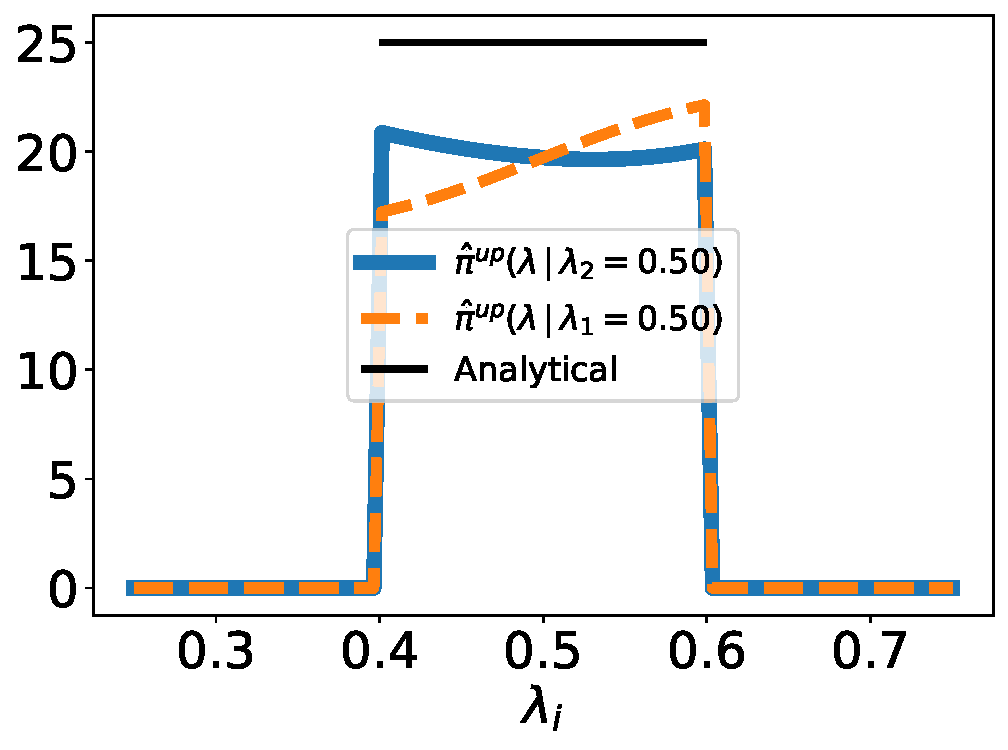
\includegraphics[width=0.5\linewidth]{./examples/identity/samp/identity_1d_conditionals_50E-2_N100_approx.pdf}
\end{minipage}
% N = 1E3
\begin{minipage}{.975\textwidth}
		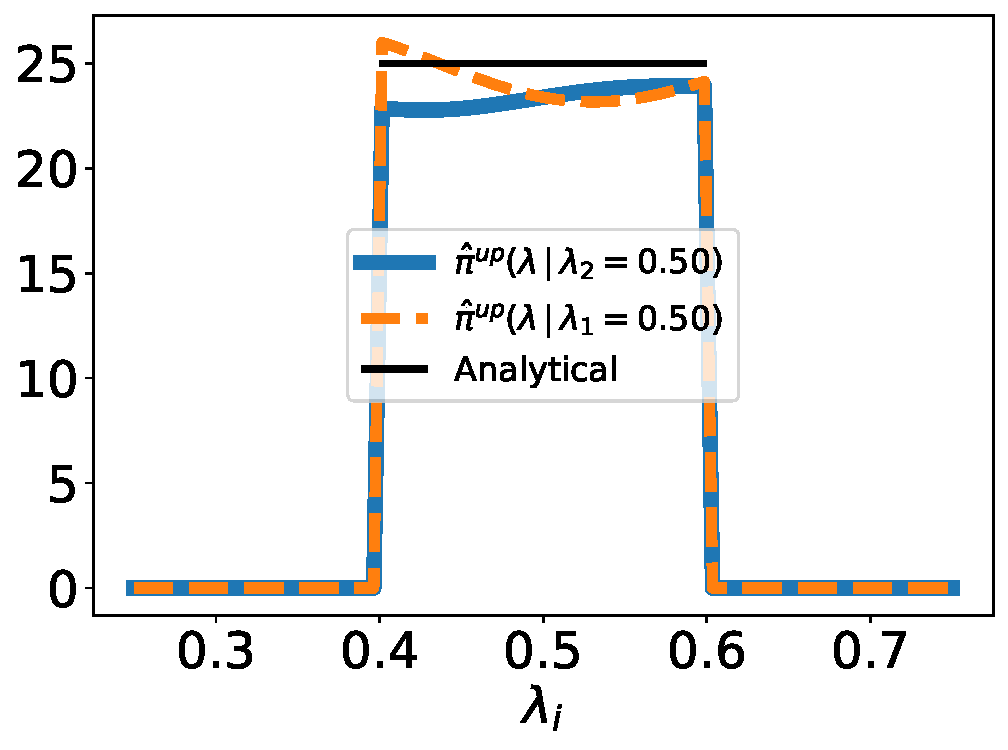
\includegraphics[width=0.5\linewidth]{./examples/identity/samp/identity_1d_conditionals_50E-2_N1000_approx.pdf}
		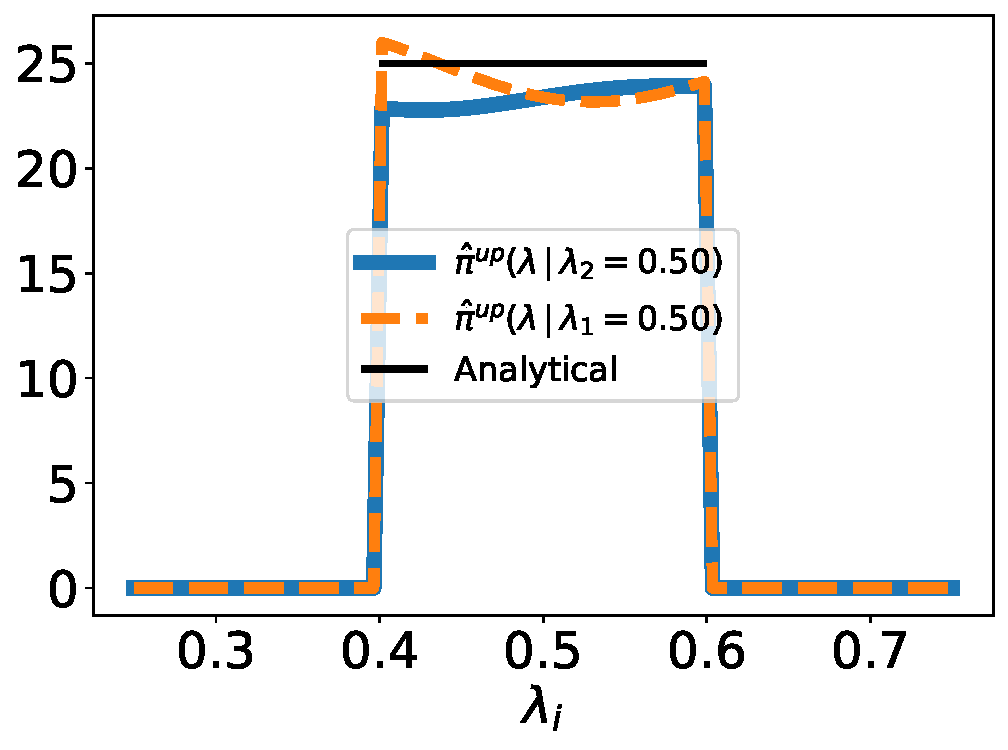
\includegraphics[width=0.5\linewidth]{./examples/identity/samp/identity_1d_conditionals_50E-2_N1000_approx.pdf}
\end{minipage}
% N = 1E4
\begin{minipage}{.975\textwidth}
		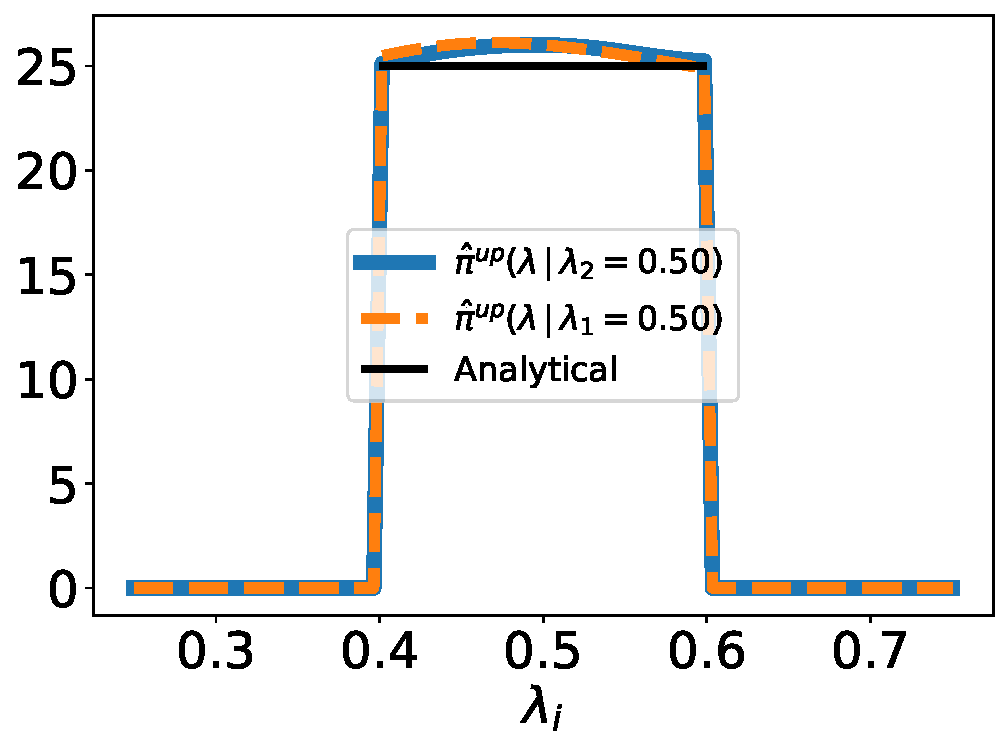
\includegraphics[width=0.5\linewidth]{./examples/identity/samp/identity_1d_conditionals_50E-2_N10000_approx.pdf}
		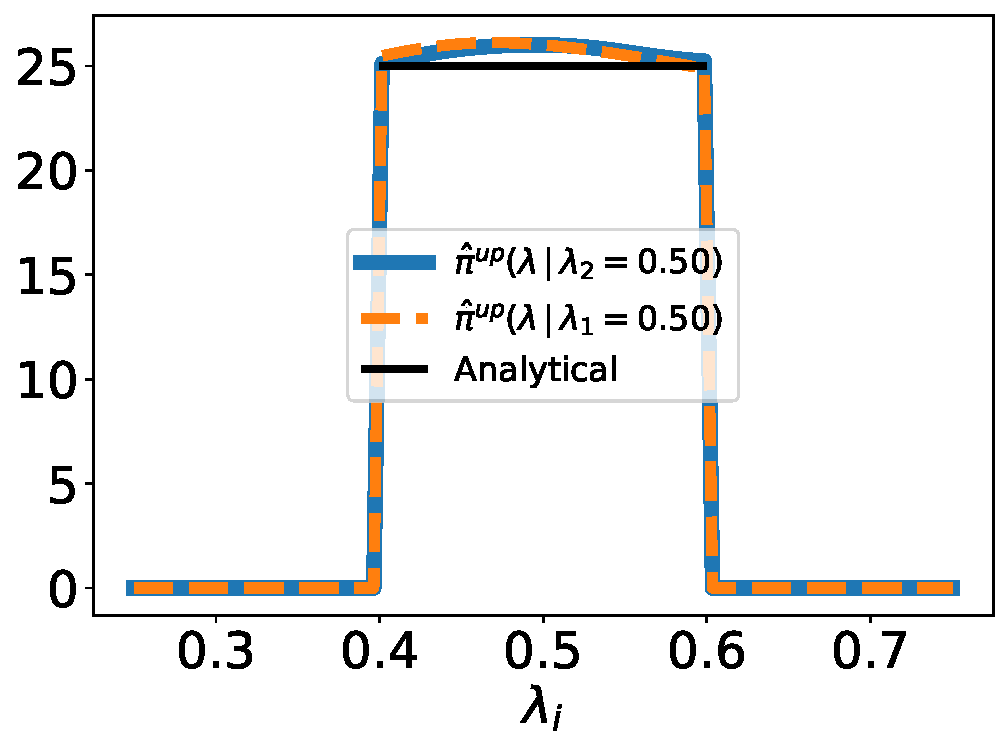
\includegraphics[width=0.5\linewidth]{./examples/identity/samp/identity_1d_conditionals_50E-2_N10000_approx.pdf}
\end{minipage}
\caption{
(Left): $\param_1=0.5$ conditional.
(Right): $\param_2=0.5$ conditional.
(Top to Bottom): Conditional for $\updated$ solutions for  $\nsamps=1E2, 1E3, \text{and} 1E4$ random samples.
}
\label{fig:identity_sampling_conditionals}
\end{figure}

Qualitatively speaking we find that the estimate of the density improve as more samples are used, but at all sample sizes, the support of the density is correctly identified, which we can see by the sharp lines in Fig~\ref{fig:identity_sampling_conditionals} and \ref{fig:ex:identity_sampling_approx}.

The sample-based method trades one source of accuracy for another.
When estimating boundaries of a set which represents an equivalent class of solutions is important, the sample best method provides a compelling alternative to be set based method.

However, we know that this is not without its pitfalls, as density estimation in high dimensions can become prohibitively prone to error.

% \FloatBarrier


%%%%%%%%%%%%%%%%%%%%%%%%%%%%%%%%%%%%%%%%%%%%%%%%%%%%%%%%%%%%%%%%%%%%%%

% \section{Illustrative Examples}\label{sec:ch02-examples}
% In some examples, an analytic, closed-form expression for the QoI map is used.
% In these examples, term (E1) in Eq.~\eqref{eq:set-triangleineq} is identically zero.
% Furthermore, since the probabilities we introduce on $\dspace$ in the numerical results are uniform and our maps linear, the densities can be described analytically with a characteristic function.
% In this event, the solution $\paramP$ to the SIP is given exactly by a change of variables formula and its support can be specified exactly.
% By inverting characteristic functions, the solutions are also be members of this same family of functions if the choice of \emph{ansatz} (or \emph{initial density}) is taken to be uniform over $\pspace$.
% 
% Such simplifications in the examples considered here allow us to study the DCI method for a class of functions for which a solution is readily available, and serves as a requisite testing ground before advancing to more nuanced problem definitions.
% In a sense, these are both ``unit'' (and ``regression'') tests for various aspects of the computational algorithms (and entire algorithms, respectively).
% We present a brief overview of the factors that influence our practical ability to accurately approximate $\paramP$ and $\updated$ using finite sampling.
% 
% For the set-based approach discussed in \ref{sec:ch02-set}, $\ndiscs$ is chosen independent of $\nsamps$ so that (E3) = $d(\PP_{\pspace, \ndiscs}, \paramP)$ from \ref{sec:set-error} is sufficiently small or eliminated entirely.
% In other words, the decision about how to discretize the uncertainty in $\dspace$ is made a priori to cater to some problem specifications.
% We choose to impose uniform distributions on $\dspace$ so that the set-valued analog to $\observed$ is perfectly described with $\ndiscs=1$.
% Elimintating this variable allows for a better comparison between the set- and sample-based approaches.
% Therefore, we focus our attention on the source of error introduced by the primary contribution of error in Eq.~\eqref{eq:set-triangleineq}:  discretizing the parameter space, which is represented by the term (E2) = $d(\PP_{\pspace, \ndiscs, \nsamps}, \PP_{\pspace, \ndiscs})$.
% The number of samples fundamentally limits the characterization of events due to the resulting simple-function approximation of the density $d\paramP / d\pmeas$, which we compare to $\updated$ from the sample-based approach.
% Since there is no error introduced from discretizing $\pspace$ in the sample-based approach from \ref{sec:ch02-sample}, the primary contribution of error in this approach comes from approximating the push-forward density in situations where an analytical $\predicted$ is not known.
% 
% \FloatBarrier
% 
\subsection{Exponential Decay}\label{ex:decay-set-sample}

To demonstrate the qualitative differences in the solutions provided by the set-- and sample--based methods for a nonlinear problem, we consider an exponential decay problem with uncertain decay rate and initial condition (which are paired to form the 2-D vector $\param$):
$$
\begin{cases}
  \frac{\partial u}{\partial t} & = \param_1 u(t), \\
  u(0) &= \param_2.
\end{cases}
$$

The solution is described by
\begin{equation}
  u(t;\param) = u_0\exp(\param_1 t), \; u_0 = \param_2 ,
\end{equation}

and a nominal value of $\param = 0.5$ is used to simulate the system.
We take a single observation at $t=0.5$s and assume a uniform density with interval length $0.2$ centered at $u(1,0.5)$ to represent the uncertainty in the measurement equipment.
We assume a uniform ansatz / initial density over the unit domain.
We use $N=50$ parameter samples to establish a coarse solution in Figure~\ref{fig:heatrod-sol-ex1}.


\begin{figure}
\begin{minipage}{.475\textwidth}
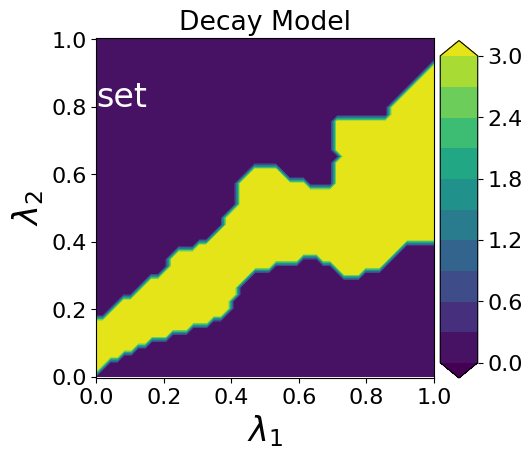
\includegraphics[width=\linewidth]{examples/fig_decay_q1/DecayModel--set_N50_em.png}
\end{minipage}
\begin{minipage}{.475\textwidth}
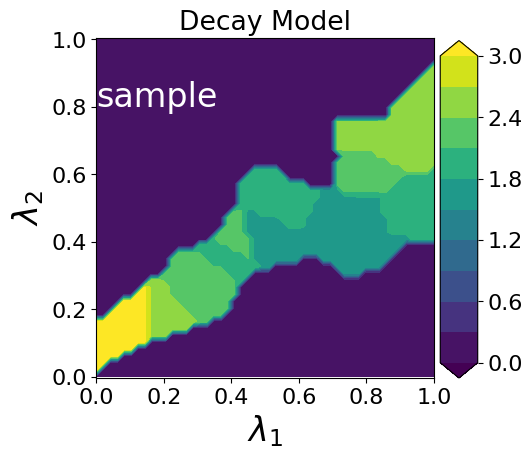
\includegraphics[width=\linewidth]{examples/fig_decay_q1/DecayModel--sample_N50_mc.png}
\end{minipage}
\caption{Observation taken at $t=1$s. The inverse image of the reference measure for set-based (left) and sample-based (right) solutions for $\nsamps=50$ parameter samples.}
\label{fig:heatrod-sol-ex1}
\end{figure}

The decay rate $\param_1$ shows little reduction in uncertainty overall.
If one were to look at marginals of the components of $\param$, it would not appear as if much was learned.
However, the relationship \emph{between} these two quantities has very certainly been elucidated by the solution of the inverse problem.
Where once $\pspace$ was a rectangular region, the set of possible parameters has been reduced to a diagonal band.
The sample-based approach, especially at this low sample size (density estimation in 2-D at $50$ samples is a stretch), has some visible downsides.
It does not capture the equivalence--class nature of the solution set the way the set--valued one does, which benefits from using $\ndiscs=1$ (aligning with the choice of uniform observed density).


We address what would occur had we been able to observe earlier in time at $t=0.5$ by showing the associated solutions under the same experimental conditions in \ref{fig:heatrod-sol-ex2}.
There is a marked reduction in uncertainty, as several regions of $\pspace$ have been ruled out from consideration.


\begin{figure}
\begin{minipage}{.475\textwidth}
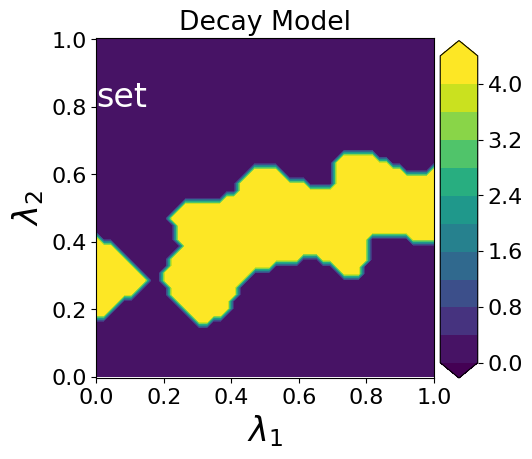
\includegraphics[width=\linewidth]{examples/fig_decay_q2/DecayModel--set_N50_em.png}
\end{minipage}
\begin{minipage}{.475\textwidth}
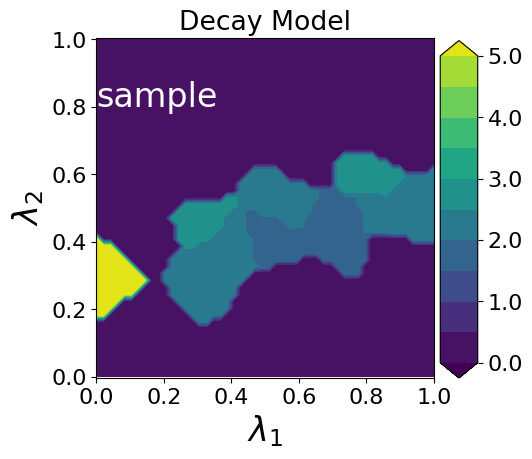
\includegraphics[width=\linewidth]{examples/fig_decay_q2/DecayModel--sample_N50_mc.png}
\end{minipage}
\caption{Observation taken at $t=0.5$s. The inverse image of the reference measure for set-based (left) and sample-based (right) solutions for $\nsamps=50$ parameter samples.}
\label{fig:heatrod-sol-ex2}
\end{figure}


Observing earlier in time helps especially in reducing the (marginal) values for the initial condition $\param_2$, while the rate $\param_1$ is still to some degree able to take any values in its original domain.
Both solution types suffer from discretization error, as evidenced by the break in the contour structure.
By comparison to \ref{fig:heatrod-sol-ex1}, there is more more confidence in the solution (represented by the reduced support of the image).

However, at $\nsamps=50$, the sample--based approach struggles to assign uniform probability to different contour events.
This may suggest that in situations with very limited model evaluation budget and set-valued solutions involving uniform uncertainties in measurements, the set-valued approach may serve a useful purpose.

% 
% \FloatBarrier
% \subsection{1D Heat Rod}\label{ex:heat-set-sample}

Consider the one-dimensional heat equation with homogeneous Neumann boundary conditions on the unit interval:

\begin{equation}
\begin{split}
\rho c \frac{\partial T}{\partial t} = \nabla \cdot ( \kappa \nabla T) + f(x), \quad & x\in (0,1), t\in (0,1) \\
f(x) = A e^\frac{- (x-0.5)^2}{w} \Chi_{[0,0.5]}(t)
\end{split}
\end{equation}
\emph{Alternative setup: }

\begin{equation}
\begin{cases}
\rho c \frac{\partial T}{\partial t} = \nabla \cdot ( \kappa \nabla T) + f(x,t), & \text{if } x\in \Omega \\
\frac{\partial T}{\partial \vec{n}} = 0 & \text{if } x\in \partial \Omega
\end{cases}
\end{equation}
where $\Omega = (0,1)\times (0,1)$ is the space-time interior and $f(x,t) = A e^\frac{- (x-0.5)^2}{w} \Chi_{[0,0.5]}(t)$.

Here, we interpret the following problem as heating the middle of an infinitesimally thin unit-length rod for half a second with the heat-source modeled by a Gaussian curve with amplitude $A=50$ and variance of $w=0.05$.
The rod is subdivided in two, and each half has an uncertain thermal diffusivity $\kappa \in [0.01, 0.2]$.
This yields a two-dimensional parameter space $\param = (\param_1, \param_2) \in [0.01, 0.2]\times [0.01, 0.2]$, where $\param_1$ represents the thermal diffusion on the left-half and $\param_2$ is the $\kappa$ for the right half.

\begin{figure}[h]
\begin{minipage}{.475\textwidth}
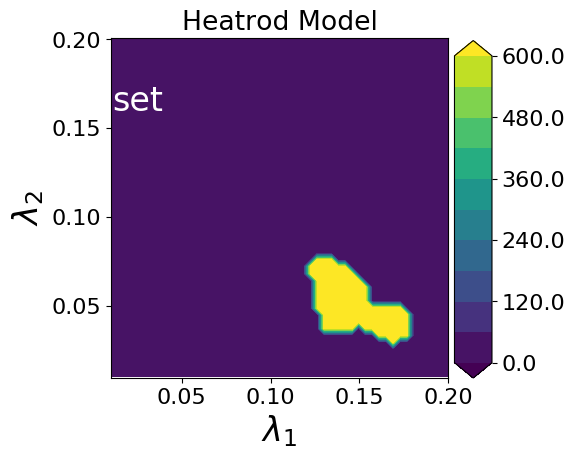
\includegraphics[width=\linewidth]{examples/fig_heatrod_q1/HeatrodModel--set_N50_em.png}
\end{minipage}
\begin{minipage}{.475\textwidth}
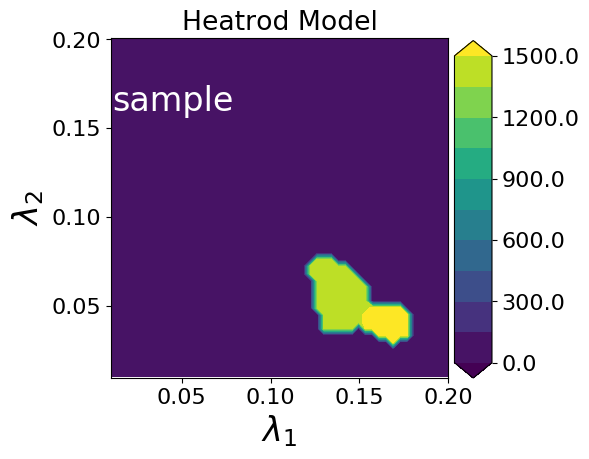
\includegraphics[width=\linewidth]{examples/fig_heatrod_q1/HeatrodModel--sample_N50_mc.png}
\end{minipage}
\caption{The inverse image of the reference measure for set-based (left) and sample-based (right) solutions for $N=50$ parameter samples.}
\label{fig:heatrod-sol-ex}
\end{figure}


\chapter{\uppercase{Computational Framework} \label{chapter:02}}

\section{Towards a Reproducible Thesis}\label{sec:reproducibility}

\subsection{Motivations}\label{sec:motivations}
In some respects, the practice of writing software has diverged from the motivations of an academic researcher.
The latter seeks to generate new knowledge and may write a set of example scripts/programs to demonstrate some novel idea or method.
By contrast, the motivations of a software engineer are related to resiliency.
Not only must they ensure the code works as expected given a myriad of ways users may interact with it, but it is necessary to write the code in a manner compatible with maintaining it into the future.
Much of the work of writing ``good software'' is concerned with writing appropriate documentation to express the intended usage and logic underlying architectural decisions.
There are many ways to write a functioning program to demonstrate a proof-of-concept, but creating something that is \emph{user-friendly}, guaranteed to be free of mistakes, and scales across different computational environments/resources requires an entirely different approach.

Decisions made early in the software design cycle have lasting impacts on future features and functionality.
Rigor is added to libraries through the writing of \emph{unit tests}, and use of \emph{continous integration} ensures that the download and installation process is predictable and reproducible.
Code that only runs on the author's computer is impractical, since any thorough critique requires independent verification.
Without proper context and architecture, new ideas that are implemented in programs are unlikely to be adopted.


This thesis is concerned not only with a demonstration of novel mathematical content\---showcasing new ways to make inferences from noisy data in a novel Data-Consistent framework\---it also serves to document the process of ensuring that the work is \textbf{fully reproducible}.
In mathematics, reproducibility is ensured through the use of proofs, which motivate the original work presented here.
However, as the title of this thesis suggests, much of the focus is actually on the computational implementation of the novel research into Data Consistent Inversion, studying the impact of using computers to perform the task of making conclusions based on data.
Mathematics is implemented on computers through software.
We are therefore concerned with ensuring the expected functionality of that software, which aligns with our training as mathematicians; we care deeply about making sure things are rigorous.

In short, we want to make sure that theory aligns with practice, and that both live up to high standards of intellectual scrutiny.
Every computational result, illustrative figure, table, plot, etc. presented in this thesis is associated with the scripts that generate them, and are included in the  repository for this document [TK - cite].
It is written in \LaTeX~(which is itself a programming language), and presents its own software dependencies in addition to those required to run the scripts to generate the images and tables.
To address this concern, we leverage \emph{Travis}, a continuous integration service [TK-cite], to ensure that all figures can be generated and the \LaTeX\, document compiles into a PDF.

The same care is taken to ensure the reproducibility of all numerical results based on software.
An \emph{image} that contains a fully pre-built Linux software environment within which one can compile the thesis and run the code is available through the Docker Cloud registry [TK -cite].
The latter enables the ability to generate this thesis document in its entirety on any software platform that supports Docker (Windows, MacOS, Linux).
A cloud service called Binder [ TK - cite mybinder.org] allows one-click deployments in any web-browser, removing the need for any installation whatsoever for anyone wanting to reproduce the contents of this document.



\section{Software Contributions}\label{sec:software-contributions}

As discussed in \ref{sec:motivations}, the entirety of the mathematical content presented has been incorporated into freely available open-source software, including this document.
The novel mathematical developments that have gone into this work are all reflected in various modules and sub-modules as part of the BET Python package.
This software suite follows a number of industry best-practices for code-coverage (\ref{sec:code-coverage}) and continuous integration (\ref{sec:continuous-integration}), i.e. the code is well-tested (\ref{sec:unit-testing}).

A significant effort in the writing of this thesis involved learning about the art and practice of modern (open-source) software development.
The author spent most of 2019 bringing the software in-line with the latest developments in Data-Consistent Inversion.


%%%%%%%%%%%

\subsection{Software Design and Architecture}\label{sec:architecture}

Having learned a lot about software reproducibility along the way, the author made the decision to treat this thesis as a software project in its own right.
Every example, figure, table, and plot is generated by a combination of Python and Shell scripts contained inside of a public Github repository (www.github.com/mathematicalmichael/thesis).

By hosting this work on Github, corrections can be submitted as Issues, and the document can serve as a reference point for a thorough introduction on the topic of Data-Consistent Inversion.
All the requisite \LaTeX~dependencies are contained in {\tt apt.txt}, and a Jupyterlab environment usable by Binder (which can compile the document and run every example) is configured in the {\tt binder/} directory of the repository (on the binder branch).

Special care is taken to ensure that every script is at least minimally documented.
When appropriate, functions and classes are used in such a way that the same file generates several examples in this thesis.
The parameters required for the variations are passed as optional arguments, and Shell scripts + makefiles containing the exact syntax to generate each figure are included.
The makefiles are particularly useful in that they track dependencies, so if changes are made to a plotting script, running {\tt make} will re-create only the figures which leverage that changed code.


We illustrate with a specific example: to visually demonstrate the implicitly-defined sets of nearest-neighbors in two-dimensional unit domain, we rely on Voronoi-cell diagrams.
One Python file (\bashinline{images/voronoi_unit_domain.py}) contains the methods required to draw a single figure; however, there are many occasions where variation on a plot may be necessary (for example, labels, different line widths).
To accommodate the need for different variations of similar plots, we utilize the argument-parsing package \pythoninline{argparse}, part of the Python standard library, to enable command-line positional and optional arguments \footnote{We equip each function with default values so that the syntax \bashinline{python example.py} without any additional arguments will work, but specific examples rely on optional arguments to be passed accordingly.}.
We include associated (wrapper) files with descriptive names, such as \bashinline{images/make_voronoi_diagrams.sh} that repeatedly call the relevant Python file(s) and passes arguments (such as {\tt num} for ``number of samples'').
We refer the inquisitive reader to  Figure~\ref{fig:voronoi_cells} or \ref{fig:voronoi_issues} to see the Voronoi-cell diagrams generated by the following script\footnote{A \LaTeX macro has been written to allow for Python and Bash files to be displayed contextually to avoid the need to update them in two places. What is shown in the body/appendix of this work is an embedded and stylized version of the exact script that was executed to generate figures.}:

\bashexternal{images/make_voronoi_diagrams.sh}


These wrappers are called by other shell scripts which are each responsible for generating figures in different sections or specific models.
This builds something akin to a ``tool chain'' or a ``pipeline,'' a series of calls to hierarchies of scripts in order to generate the pictorial and tabular content in this work.

%%%%%%%%%%%
\subsubsection{Software Dependencies and Docker}\label{sec:docker}
[TK - brief intro to images, containers]
We document the process of how the containers which were used to generate all the results here (the {\tt bin/} directory of this thesis contains the relevant shell scripts), are generated by including the Dockerfiles for them.
This static snapshot allows us to be assured our results can be recreated on x86 architecture (theoretically in perpetuity).
The author also published versions of the relevant images compiled on ARM, and has recreated all figures on a Raspberry Pi as validation.
However, at the time of writing there exists a set of dependencies not yet implemented in an arm-based Dockerfile.
The scientific computing software (largely developed by collaborations among researchers at the national laboratories) FeNiCS, was compiled from source on ARM, as a proof-of-concept.
Generating a docker image which builds the software from source on ARM is a to-do for the author, and can already be theoretically brute-forced by copying over the requisite built-files from the host operating system\footnote{As a stopgap measure for ARM-support, the entire RaspberryPi has been backed up to an image and published online, so that all the dependencies can be resolved by switching microSD cards.}.
FeNiCS is available through conda but only on x86, and no ARM-based docker images are provided to be leveraged.


%%%%%%%%%%%
\subsubsection{Testing}\label{sec:unit-testing}
The aforementioned \emph{unit tests} provide a framework for guaranteeing the behavior of programs or individual methods when instructions are followed.
\emph{Functional tests} encompass more complicated behavior, stringing together several methods/modules to ensure code runs as its author intended, and are usually included when referring to unit testing.
``How to write a test'' is a question that depends highly on the particular functionality, but the premise is always the same.

[TK - maybe show a really basic example of a set/get method and the test for that?]

%%%%%%%%%%%

\subsubsection{Code Coverage}\label{sec:code-coverage}

Code coverage refers to the proportion of lines of code that were run during the process of testing (consisting of unit and functional tests).
The goal is not necessarily to achieve 100\% coverage, but rather to make sure that the most crucial use-cases are checked.
Generally speaking, coverage in the 75-85\% range is industry-standard.

[TK - flesh out a bit more, talk about Codecov, the specific service we use, how it won't be used for the scripts in this thesis].

%%%%%%%%%%%

\subsubsection{Continuous Integration}\label{sec:continuous-integration}

These outer-level scripts that call others are leveraged by continuous-integration (CI) services (Travis, Github Actions), that run a series of commands on behalf of the user, automating the process of testing functionality.
The familiarity with this technology was introduced as a consequence of working on BET \cite{pyBET}, the software library that originally implemented the set-based approach discussed in \ref{sec:ch02-set}.
The use of CI in BET is similar to that of many software packages written in Python; unit tests are run in some framework (\pythoninline{nose} for BET at first, eventually migrated to \pythoninline{pytest} at the author's insistence), and a successful run triggers a webhook that communicates with the software repository host (Github) to validate changes. Github receives messages from the CI service and shows a visual indicator of the status of the work done.

Github Actions came out [TK - date] during the final year of writing this thesis, and provided a convenient way to orchestrate and check on the status of continuous-integration and deployment

\subsubsection{Continuous Deployment to DockerHub and PyPi}
Give an intro to CD principles. Relevant here because the {\tt mud} Python library which implements the analytical expressions presented here and is a shared library for many of the examples, particularly in Chapter~\ref{chapter:mud}.
This library leverages all of the aforementioned principles and components, and additionally automatically publishes to the PyPi registry, allowing anyone to {\tt pip install mud} to resolve \emph{most} of the dependencies of novel contributions presented here.
A similar effort is underway for CD in BET, though the version(s) used here have already been published ({\tt pip install bet}).
Even as changes are made after this thesis is published, readers of this work can rest assured that the results are still reproducible because Github Actions validates all of it on a weekly schedule.
As soon as reproducibility problems surface, the author will be notified so they can be addressed, and the latest build status of the project is visible to the public.

\subsection{Background and Motivation}
The open-source software package BET was developed actively from 2012-2015 under grant [TK grant-NSF+DOE].
It was originally written in Python 2.7 and is currently administered by the Computational Hydrology Group at the University of Texas: Austin through their UT-CHG GitHub group [TK - cite Github].
The initial purpose of this open-source software package was to implement the methods first described in [TK - cite BET papers] for the description and solution of stochastic inverse problems summarized in Section~\ref{sec:ch02-set}.
In the intervening years since its original publication in [TK - date of first release, cite Github], the BET package has seen two major releases and the incorporation of several sub-modules (e.g. the functions in {\tt sensitivity} implement much of the original research performed by Dr. Walsh [TK - cite Scott]).


\subsection{Upgrades, Updates, and Features}
Since the last major release [TK - cite latest release], the Python community announced the end of long-term support for Python 2 [TK - cite announcement].
Several of the dependencies in BET have been actively developed in Python 3 with no updates to the Python 2 analogs, which necessitated an upgrade to allow the package to be a usable contribution to open source software.
The work summarized in Section~\ref{sec:ch02-sample} was implemented in Python 3 independently by the author through the release of the ConsistentBayes package.
Since that code was used for many of the preliminary results for this work, it made very little sense to re-implement them in Python 2 for BET given the recent trends in community development.
With funding made available through the NSF [TK - cite grant], the opportunity to upgrade BET to Python 3 allowed the library to avoid falling into disuse by relying on an unsupported language.


\subsubsection{Version 2.1.0}
The upgrade to Python 3.4+ began in January 2019 as a first step to incorporate the new sample-based method into BET.
It was completed in late February.
Major (minor? version? TK) release 2.1.0 [TK - put in release] was designed to provide backwards-compatibility with the Python 2.7 version.
Future installations (starting in 2020) will not limit the versions of some core dependencies in order to accommodate backwards-compatibility with Python 2 (e.g. {\tt numpy}, {\tt scipy}), since this would likely downgrade previously installed software for end-users.


\subsubsection{Version 2.2.0}
Several releases of BET (after the upgrade to Python 3 in v2.1.0), incorporated developments that will be discussed herein.
[TK - i have no recollection what the significance of this was]

\subsubsection{Version 2.2.1}
Major bugfix for parallel testing allowed tests to pass for more than 2 processors.
For some tests, this involved changing the setup parameters to ensure the problem was large enough to break up onto up to 8 processors.
For others, significant changes had to be made to structure to allow for proper saving and loading of files in parallel.


\subsubsection{Version 2.3.0}
This release incorporated the sampling-based approach discussed in Section~\ref{sec:ch02-sample}.
However, it never made it to the master branch of the project due to architectural changes in BET.
It was used for generating many of the results in this thesis initially by pointing to {\tt install\_bet.sh} which pulled the specific branch, but eventually this was swapped for Version 3.0.

\subsubsection{Version 3.0}
This version implemented the sample-based approach by the introduction of new sub-classes.
It broke backwards-compatibility with much of the code written for this work.
[TK - point to the github PR that eventually upgrades the examples (hopefully including ones for the master's. I figure it's one or two night's work, but very low priority since I am using docker to ensure that everything can be reproduced. In fact, it's actually a testament to git + docker that I can point to code in the past and recreate the results.)]

\subsection{Examples in BET}
Basic plotting functionality of BET is demonstrated in iPython notebooks [TK - some kind of citation here], which have seen an exponential growth rate on GitHub, and can be edited by the end-user to work with different plotting library versions and backends.
These notebooks were originally created to reflect the example suite in BET (which were {\tt .py} files), but later they were migrated into a separate repository BET-examples to allow for better organization.
In the new framework, each notebook functions as an independent example.
Several of these notebooks were adapted from the example code in this thesis repository.


[TK - for ch4 purposes...]
Talk about the BET module that computes metrics.
Discuss testing, show sample of usage (disconnected from skewness, high-level).

\FloatBarrier
